\section{Implementation}
\label{sec:implem}
\addcontentsline{toc}{chapter}{Implementation}

The model and application we are studying are new to the literature and therefore our implementation of the model has also been built from scratch.  For our simulations we have build a NetLogo application that allows the user to simulate the outcome of the previously described model. The interface also allows the creation of custom worlds and the simulation (in single run or batch mode) of different scenarios in which all or part of the four primary variables are modulated. A typical world view is presented in fig. \ref{fig:world}. 

\restylefloat{world}
\begin{figure}[H]
\centerline{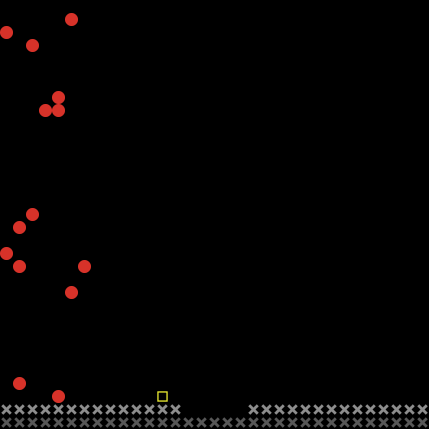
\includegraphics[scale=0.45]{images/world}}
\caption{An initial setting of the world in which the simulation takes place. The red dots denote randomly placed bots, the \emph{X} marked places show obstacles and the yellow box is the object that needs to be transported to the other end of the world.}
\label{fig:world}
\end{figure}

Each of the entities involved (i.e. bots, objects and obstacles) are defined as agents within NetLogo. The objects have individual weights, the bots are considered to all have a pushing power of one. 

At each time step, the operations in listing \ref{lst:mainLoop} are performedy by the system. First, a bot is activated randomly and is allowed to perform a movement action based on the implemented rules described previously in section \ref{sec:model}. Then all the bots are allowed to make a pushing action, where only the bots that have a box in the immediate vicinity are activated. These proceed to the pushing phase described in listing \ref{lst:pushing}. Here the bot finds what the pushing power required for the next obstacle(s) and depending on how many bots can help push the object, it may decide to do so or wait for a new time to act (when perhaps it will be supported by the required number of bots). During the entire process both the bots and the boxes are affected by gravity. This activity is performed at each time step and moves the bot to the lowest possible location to the ground that has the same $x$ coordinate within the world.

\lstinputlisting[label=lst:mainLoop,caption=The operations performed at each time step.]{code/main-loop.txt}

\lstinputlisting[label=lst:pushing,caption=The actions performed when pushing a box.]{code/pushing.txt}
